\serie{Solutions d'une équation}


\begin{exercice}[Vocabulaire]

\[ 9x + 2 = 39  \qquad \qquad 4y + 8 + 5y = y^2 + 3 \]

Pour chaque équation, indique : 
\begin{colenumerate}{1} 
\item l'inconnue ;
\item le ou les termes comportant l'inconnue ;
\item le ou les termes constants ;
\item les membres de l'équation.
\end{colenumerate} 
\end{exercice}




\begin{exercice}[Être solution ou non ?]

\begin{colenumerate}{1} 
\item Le nombre $-5$ est-il solution de l'équation $5 -4x = 29$ ? Et le nombre $-6$ ?
\item Le nombre 8 est-il solution de l'équation $5y -3 = 2y + 2$ ? Et le nombre $-3$ ? Et $\dfrac{5}{3}$ ?
\item Parmi les nombres 5, $-3$ et 2, lesquels sont solutions de l'équation $z^2 + z -6 = 0$ ?
\end{colenumerate} 
\end{exercice}



\begin{exercice}[]
Parmi les équations suivantes, quelles sont celles qui admettent pour solution celle de l'équation $7y + 5 = 3y + 8$. Justifie.

\begin{colenumerate}{2} 
\item 4y + 5 = 3y + 8
\item 7y = 3y + 4
\item 14y + 10 = 6y + 16
\item 7y -5 = 3y + 1
\end{colenumerate} 
\end{exercice}



\serie{Résoudre des équations}


\begin{exercice}[Équations du type $x + a = b$]

Résous les équations suivantes :

\begin{colenumerate}{2} 
\item $x + 6 = 8$
\item $t -7 = 3$
\item $y + 11 = 10$
\item $1 + x = -2$
\item $t -5 = -3$
\item $x -5,3 = -3,2$
\item $y + 15,7 = -30$
\item $-5,4 + t = 4,85$
\item $x + 7 = -1,2$
\item $y -59,7 = -100$
\end{colenumerate} 
 
\end{exercice}

\begin{exercice}[Équations du type $ax = b$]

Résous les équations suivantes :

\begin{colenumerate}{2} 
\item $3x = 9$
\item $5y = 3$
\item $4z = -7$
\item $-2z = -8$
\item $7x = 4$
\item $-y = -7,2$
\item $-y = 15,7$
\item $4,4z = 0$
\item $2,7x = -1,2$
\end{colenumerate} 
\end{exercice}

\begin{exercice}[]Équations du type ax + b = 0

\begin{colenumerate}{1} 
\item Résous les équations suivantes :
    \subitem $4x -12 = 0$
    \subitem $2x -3 = 0$
    \subitem $4x + 1 = 0$
    \subitem $2 -3x = 0$
\item On considère l'équation $ax + b = 0$ où $a$ et $b$ sont des nombres relatifs, $a$ étant non nul. Exprime la solution $x$ de cette équation en fonction de $a$ et de $b$.

Vérifie alors tes résultats précédents.

\item Déduis-en directement la solution de chacune des équations suivantes : 
    \subitem $2x + 8 = 0$
    \subitem $3x -1 = 0$
    \subitem $11x + 1 = 0$
    \subitem $2 -7x = 0$
    \subitem $7x + 8 = 0$
    \subitem $2,8 -4x = 0$
\end{colenumerate} 
\end{exercice}



\begin{exercice}[Méli mélo]

\begin{colenumerate}{1} 
\item Résous les équations suivantes :
    \subitem $7x = 28$
    \subitem $7 + x = 28$
    \subitem $-7x = -28$
    \subitem $7x = -28$
    \subitem $7 -x = 28$
    \subitem $x -7 = -28$
    \subitem $7 + x = -28$
    \subitem $x -7 = 28$
    \subitem $-7x = 28$
    \subitem $7 -x = -28$
\item Regroupe les équations qui ont la même solution et explique pourquoi.
\item Sans faire de calculs et en justifiant, donne la solution de chacune des équations suivantes :
\[ -x -7 = 28	\qquad \qquad 	-x -7 = -28 \]
\end{colenumerate} 
\end{exercice}




\begin{exercice}[Équations du type $ax + b = c$]

Résous les équations suivantes :

\begin{colenumerate}{2} 
\item $2x -2 = 2$
\item $3z -10 = 11$
\item $1 -y = 0$
\item $1 + 5x = -39$
\item $2 + 3z = 9$
\item $6 -y = -2,3$
\item $7 -3x = -22$
\item $5 + 6z = -11$
\item $-x -9 = 11,2$
\item $9,7y -5,7 = -1,7$
\end{colenumerate} 
\end{exercice}




\begin{exercice}[Solutions particulières]

Résous les équations suivantes :

\begin{colenumerate}{3} 
\item $6x = 6x + 1$
\item $3n = 0$
\item $0y = 0$
\end{colenumerate}
\end{exercice}




\begin{exercice}[Équations du type $ax + b = cx + d$]

Résous les équations suivantes :

\begin{colenumerate}{2} 
\item $5x = 3x + 3$
\item $8x = 12x + 4$
\item $4 -7y = 10y$
\item $7x + 1 = -4 -x$
\item $2 + 3x = 7 -3x$
\item $5 + 6x = -x -9$
\item $11x + 3 = 8x + 7$
\item $5,5x + 1,5 = 9x + 6$
\item $7 -3,3x = 2x -9,7$
\item $5,1 -x = -8x + 1,7$
\end{colenumerate} 
\end{exercice}




\begin{exercice}[Plus complexe]

Résous les équations suivantes :

\begin{colenumerate}{1} 
\item $4(x + 5) = 10x + 3$
\item $3(x -2) = 6(x + 4)$
\item $7x -(5x + 3) = 5(x -3) + 2$
\item $7(n + 2) -3 = 25 -(3n + 4)$
\item $4y + 3(4y -2) = 3(y + 1)$
\end{colenumerate} 
\end{exercice}


\serie{Problèmes}





\begin{exercice}[Dans ma classe]
Il y a 28 élèves. Le jour où Lucas était absent, il y avait deux fois plus de filles que de garçons.

Combien y a-t-il de filles dans ma classe ?
\end{exercice}




\begin{exercice}[Nombres consécutifs]

\begin{colenumerate}{1} 
\item Trouve trois nombres entiers consécutifs dont la somme vaut 513.
\item Peux-tu trouver trois nombres entiers consécutifs dont la somme vaut 200 ? Justifie.
\item Trouve quatre nombres entiers consécutifs dont la somme vaut 1 254.
\item Invente un problème pour trouver cinq nombres entiers consécutifs.
\end{colenumerate} 
\end{exercice}



\begin{exercice}[Argent de poche]
Mes parents me donnent de l'argent de poche depuis que j'ai 12 ans. Mon père m'a donné la première année 5\,€ par semaine. Il augmente cette somme tous les ans de 5\,€. Ma mère me donne le double de mon père.

À quel âge aurai-je 60\,€ par semaine ?
\end{exercice}

\begin{exercice}[Commerce de glaces]
Un marchand dépense 75\,€ par semaine pour confectionner ses glaces. Sachant qu'une glace est vendue 2,50\,€, combien doit-il vendre au minimum de glaces dans la semaine pour avoir un bénéfice supérieur à 76\,€ ?
\end{exercice}




\begin{exercice}[Programmes de calculs]
Alice et Bertrand affichent un même nombre sur chacune de leur calculatrice. 
\begin{cadre}
Alice multiplie le nombre affiché par 3 puis ajoute 4 au résultat obtenu.
\end{cadre}
\begin{cadre}
Bertrand multiplie le nombre affiché par 2 puis ajoute 7 au résultat obtenu.
\end{cadre}
 
À la fin, ils s'aperçoivent que leurs calculatrices affichent exactement le même résultat. Quel nombre ont-ils affiché au départ ? 
\end{exercice}




\begin{exercice}[Le nombre cherché]
Joey pense à un nombre. Il lui ajoute 11, multiplie le tout par 3 et au résultat obtenu il retranche 3. Joey obtient 51.

Quel est ce nombre de départ ?
\end{exercice}




\begin{exercice}[Problème d'âges]
Mickaël a 18 ans et son père a 46 ans.

Dans combien d'années le père de Mickaël aura-t-il le double de son âge ?
\end{exercice}



\begin{exercice}[Moyenne de Maths]
Hervé a obtenu lors des trois premiers devoirs les notes suivantes : 8 ; 5 et 14.

Quelle note minimale doit-il obtenir au dernier devoir pour avoir la moyenne ce trimestre ?
\end{exercice}



\begin{exercice}[Sécurité routière]

\begin{cadre}

\vspace{.5em}

\[E_c = \dfrac{1}{2} MV^2\]

où $M$ est la masse (en kg) et $V$ est la vitesse (en m/s).

\vspace{1em}

\[E_p = Mgh\]

où $M$ est la masse (en kg), $g$ = 9,81 (en N/kg) et $h$ est l'altitude (en m).

\vspace{.5em}

\end{cadre}


Pour évaluer les forces d'impact, on calcule l'énergie cinétique $E_c$ (énergie liée au mouvement) et l'énergie potentielle de pesanteur $E_p$  (énergie liée à l'altitude).

\begin{colenumerate}{1} 
\item Un véhicule de 900 kg roule à 60 km/h. Sachant que 60 km/h $\approx$ 16,7 m/s, calcule son énergie cinétique $E_c$.
\item À quelle hauteur doit être placé ce véhicule pour que son énergie potentielle $E_p$ soit égale à l'énergie cinétique trouvée en \textbf{1)} ?
\item Reprends les questions \textbf{1)} et \textbf{2)} avec un véhicule qui roule deux fois plus vite.
\end{colenumerate} 
\end{exercice}



\begin{exercice}[Partage...]
On partage une certaine somme entre trois personnes. La première reçoit 2\,160\,CHF, qui représentent $\dfrac{2}{5}$ de la somme. La deuxième reçoit $\dfrac{1}{3}$ de la somme, et la dernière reçoit le reste. Quelle est la somme partagée, et quelles sont les parts des deux dernières personnes ?
\end{exercice}



\begin{exercice}[]
Deux-tiers des trois-quart de la moitié du prix de vente d'une voiture représentent 5\,000\,CHF. Quel est le prix de vente de la voiture ?
\end{exercice}



\begin{exercice}[]
J'ai 180\,€ de plus que toi. Si je te donnais 41\,€ alors j'aurais deux fois plus d'argent que toi. Combien avons-nous chacun ?
\end{exercice}

\begin{exercice}[Pièces]
Avec 25 pièces, toutes de 1\,€ et 2\,€, j'ai une somme de 38\,€.
Combien ai-je de pièces de chaque sorte ?
\end{exercice}



\begin{exercice}[Le concert]

La grande Halle d'Auvergne peut accueillir 8\,500 spectateurs. Lors d'un concert, toutes les places debout à 25\,€ et toutes les places assises à 44\,€ ont été vendues. Le montant de la recette était ce soir-là de 312\,725\,€. 
Quel était le nombre de spectateurs debout ? 
\end{exercice}




\begin{exercice}[Cinéma]

Le ciné-club d'un village propose deux tarifs :

Tarif A : une carte d'adhésion pour l'année coûtant 21 euros, puis 1,5\,euros par séance ;

Tarif B : 5 euros par séance sans carte d'adhésion.

\begin{colenumerate}{1} 
\item Calculer, pour chaque tarif, le prix payé pour 8 séances.
\item On appelle $x$ le nombre de séances. Exprimer en fonction de $x$ le prix payé avec le tarif A, puis avec le tarif B.
\item Quel est le nombre de séances pour lequel le tarif A est égal au tarif B ?
\end{colenumerate} 
 \end{exercice}



\serie{Problèmes de géométrie}




\begin{exercice}[]
On transforme un carré en un rectangle en ajoutant 7\,cm à la longueur d'un de ses côtés et en retranchant 2\,cm à la longueur d'un autre. 

\begin{colenumerate}{1} 
\item Quelles doivent être les dimensions du carré initial pour que le double de son périmètre soit égal au périmètre du rectangle ?
\item Quelles doivent être les dimensions du carré initial pour que son aire et celle du rectangle soient égales ? 
\end{colenumerate} 
\end{exercice}




\begin{exercice}[Périmètre d'un triangle]
\ImageDroite{Trouve la valeur de $z$ sachant que le périmètre du triangle ci-contre vaut 61.
Les mesures sont dans la même unité.}{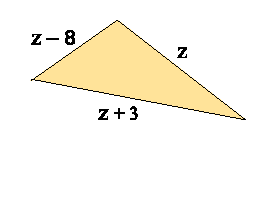
\includegraphics[width=.5\linewidth]{EqEE01}}
\end{exercice}



\begin{exercice}[Surfaces égales]
Soient le trapèze et le parallélogramme ci-dessous. Les mesures sont dans la même unité.

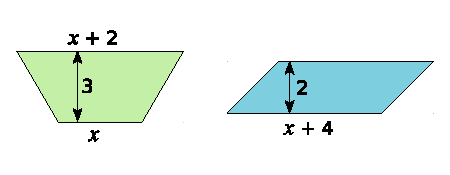
\includegraphics[width=\linewidth]{EqEE02}

Quelle doit être la valeur de $x$ pour que le trapèze ait la même surface que le parallélogramme ?

\textit{Rappel : l'aire d'un trapèze est égale à $\dfrac{(B+b)\times h}{2}$ où $B$ est la longueur de la grande base, $b$ celle de la petite base et $h$ celle de la hauteur. L'aire d'un parallélogramme est égale à $b\times h$ où $b$ est la longueur de la base et $h$ la hauteur relative à cette base.}
\end{exercice}



\begin{exercice}[Le quart du cinquième du sixième ???]

On considère trois nombres notés, dans cet ordre, $x$, $y$ et $z$. Le quart du premier est égal au cinquième du second qui est lui-même égal au sixième du troisième. De plus, la somme de ces trois nombres est égale à 600.

\begin{colenumerate}{1} 
\item Calculer $y$ et $z$ en fonction de $x$.
\item En déduire la valeur de ces trois nombres.
\end{colenumerate}
\end{exercice}
